\section{Experiment Setup}
\label{sec:experimentSetup}
After developing the prototypes, we implemented a version of the Job Simulator hands which we used as a baseline for comparison during our user evaluation. For the evaluation we decided to compare only one of the prototypes with the Job Simulator hand, which was the Physics hand.

The evaluations ran in a structured manner one tester at a time. Each person would first play through what we call the Dev World environment first with the Job Simulator hand to establish the baseline and then with the Physics hand, after which they would do the same with a more game-like environment, which we call Touchy Island. The Dev World is a small-scale environment with a few basic objects that the users can interact with in different ways. Touchy Island is more like an experience, where the player can interact with different creatures and objects on a floating island. The details of both these environments are noted below in Sections \ref{subsec:devWorld} and \ref{subsec:touchyIsland}. While experiencing the two hands in the Dev World, the users were prompted to follow a set of instructions which would guide them through the different interactions possible with the hands to make sure they noticed their features. Besides the features of the hands, the instructions also mentioned the controls, like using the trigger to close the hand. In order for the players to be able to move around the environments, which are larger than the play space of the Vive, we  implemented teleportation, which can be activated using the track pad on the controller.

\begin{figure}
\begin{itemize}[noitemsep]
\item Press the triggers to close the hands.
\item Touch immovable object.
\item Move controller deep into immovable object.
\item Hover over a grabbable object.
\item Grab a grabbable object.
\item Move around the grabbed object.
\item Hit an object with a grabbed object.
\item Throw a grabbed object.
\item Push a grabbable object.
\item Break the joint set up between two of the grabbables by grabbing one of the objects with each hand and pulling in opposite directions.
\item Lift a grabbable object without grabbing it with the triggers.
\item Teleport using the track pad on the controller.
\end{itemize}
\caption{List of actions the testers were guided through, while in the Dev World environment.}
\label{fig:listActionsDevWorld}
\end{figure}

When the testers had gone through the instructions in the Dev World for both hands, we continued to Touchy Island. In Touchy Island we would not guide them with specific instructions, but allow them to freely move around and experience the interactions possible. Sometimes we would hint at certain interactions or features of Touchy Island, if the testers hadn't discovered them within a certain timeframe, but the second environment was meant for playing with the hands, while being reminded by the possibilities presented in the first environment. In Touchy Island the testers would also first evaluate our implementation of the Job Simulator hand before moving to the Physics hand, each of which took 5 to 10 minutes. During the evaluations we would record both the screen and the testers themselves through the webcam of the computer running the tests, where permission was given. This material was saved to be able to look back at, if any issues should come up later during the analysis of the evaluations.

After the evaluations were over, we asked the testers to fill in a questionnaire, where most questions were set up like an A/B test. They would select which of the hands felt better in certain contexts or situations. An example from the questionnaire would be: "With which version did you prefer pushing things?". The full questionnaire can be found in the Appendix (\textbf{\textit{REF}}). During the evaluation, the Job Simulator hand was named Standard hand and the Physics hand was named Adaptive hand. This was to remove associations induced by the names. At the end of the questionnaire we had two questions, which were about selecting from a list of words the ones they thought fit best with the Standard hand and then with the Adaptive hand. The reasoning behind these questions were to start making the testers think about the hands using different descriptors, which we hoped would be able to lead them into the short interview and discussion we would perform afterwards with more ease.

The questionnaire was meant to make the testers start thinking about the hands and how they compared in different contexts, which would lead into an interview and discussion about the hands. When the questionnaire had been filled, we would discuss both hands and dig into why the tester preferred one hand over the other in certain contexts. The questions were guided by the answers we'd received through the questionnaire to dig deeper into the why of these preferences. During the interview, short-form notes were taken to remind us later during the analysis about what had been said in more detail. The questionnaires and the notes from the interviews form the base of our analysis. The video material ended up not being needed.

\begin{table}[h]
\centering
\caption{Test procedure for the user evaluations.}
\label{tab:testProcedure}
\begin{tabular}{lL{2cm}L{5cm}L{5cm}}
Phase & Duration & Tester & Organizer \\ \midrule \midrule
Introduction & 5 mins & & Introduce tester to test scenario and purpose. \\ \midrule
Play test & 5 mins + 5-10 mins & Test Standard hand and Adaptive hand in Dev World and Touchy Island environments. & Observe tester, guide through actions in the Dev World. \\ \midrule
Questionnaire & 3 mins &Tester fills out questionnaire & \\ \midrule
Verbal feedback & 20 mins & Answer questions about test session and discuss hands. & Ask questions about and discuss the hands. \\
\end{tabular}
\end{table}

\subsection{Dev World}
\label{subsec:devWorld}
The Dev World was created and expanded upon, while the prototypes were developed. It was originally set up to allow us to test our prototypes as they were being implemented. It originally consisted of only a floor, a large immovable cube and some small cubes on top that could be pushed around. The immovable cube was used mainly to test how the position filtering worked for the different hands allowing us to test on both large flat surfaces, but also around edges and corners which often introduce difficulties. The smaller cubes could be pushed and later, when grabbing was introduced they could also be grabbed and thrown. These features helped test how the fingers' placement looked, both before and while grabbing the objects. A punching bag was added, which was a capsule fastened by one end to its original position in the world using a joint. The punching bag can be pushed, bending around the joint position and snapping back. When users discovered the punching bag, they often started boxing for a short while without being told.

Later in the process we added a few extra things to test newer functionality implemented in the prototypes and grabbing systems. We added a long thin cylinder, which was used to test finger positioning on smaller objects and it was also used to test behavior like hitting objects with a grabbed object instead of with the hand directly. A set of cubes were also added that were connected with a joint. The joint has break forces enabled allowing the joint to break, when forces above a certain threshold is observed. If the cubes are grabbed, one in each hand, and they are being pulled apart, the joint might break. This was mainly created as a plaything that the users could interact with, but also to test the feel of pulling on objects that are stuck. The last thing added to the Dev World was a large cube, which isn't immovable, but has a very high mass. This cube was added to be able to test the effect of pushing heavy objects with the hands, especially the Physics hand. All our prototypes, with the exception of the Physics hand, has the same feeling while pushing objects of different weights, whereas the Physics hand made the users' able to get a sense of weight.

In the Dev World, all immovable objects are dark gray of color and all objects that can be pushed, grabbed or otherwise interacted with are brightly colored to show the users which are which.

\begin{figure}[h]
\centering
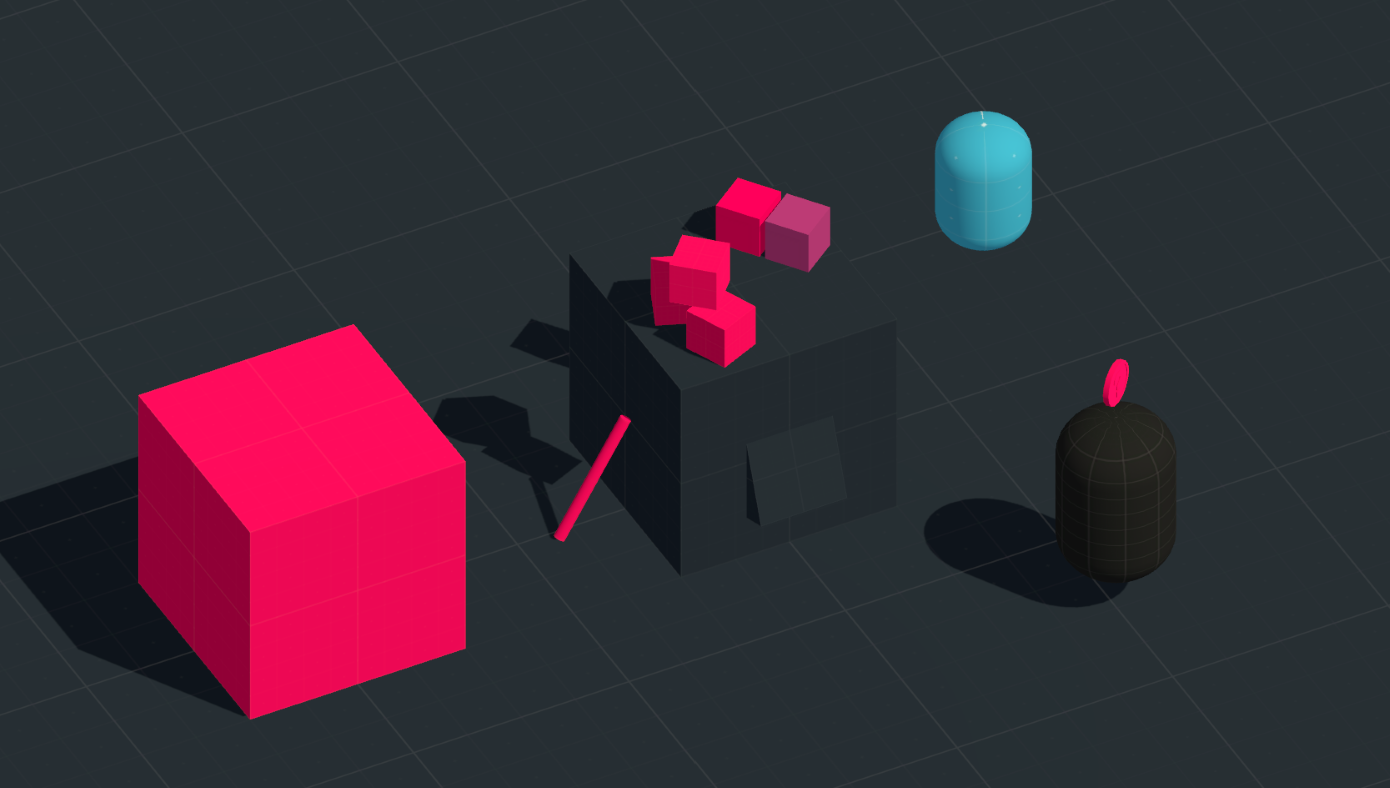
\includegraphics[width=1.0\textwidth]{Environments/devWorld.png}
\caption{An image of the Dev World.}
\label{fig:devWorld}
\end{figure}

\subsection{Touchy Island}
\label{subsec:touchyIsland}
The second environment, Touchy Island, was created for different reasons and with different goals in mind compared to the Dev World. Where the Dev World was created and developed along with the prototypes, Touchy Island was created for use during the user evaluations. Touchy Island is like a small experience or sandbox game, where the player can interact with a couple of different types of creatures and objects on a small floating island. The main idea is that the creatures all have moods and their moods are affected by their surroundings. Each of these creatures also have their own small quirks or features, which differentiates them from the other types and which would make the player interact with them differently\footnote{As part of the planning for the development of Touchy Island we prepared a design document. It contains descriptions of several of the elements that went into the final version of the sandbox, although it wasn't kept completely up to date throughout the process. The design document can be found in the appendix \textbf{\textit{(REF)}}.}. The four creature types present on the island are the Rock creatures, the Cherry creatures, the Mole creatures and the Cloud creatures.

The Rock creatures start out as small and almost cube shaped. Their shape allows them to be stacked on top of each other, if that's what the player would like to do. The player can then try to move around stacks of Rock creatures while playing a balancing game of sorts. The Rock creatures move around by rolling onto one of the sides it's not currently standing on, like a dice rolling. This also means that they sometimes lie on their sides, their backs or even their faces. The Rock creatures are the only ones that age and grow. Over time the Rock creatures will grow old. When this happens, they will be enveloped in a cloud of smoke and they will emerge larger and with crystal hair and a mustache. Rock creatures are also the only creatures that die of old age.

\begin{figure}[h]
\centering
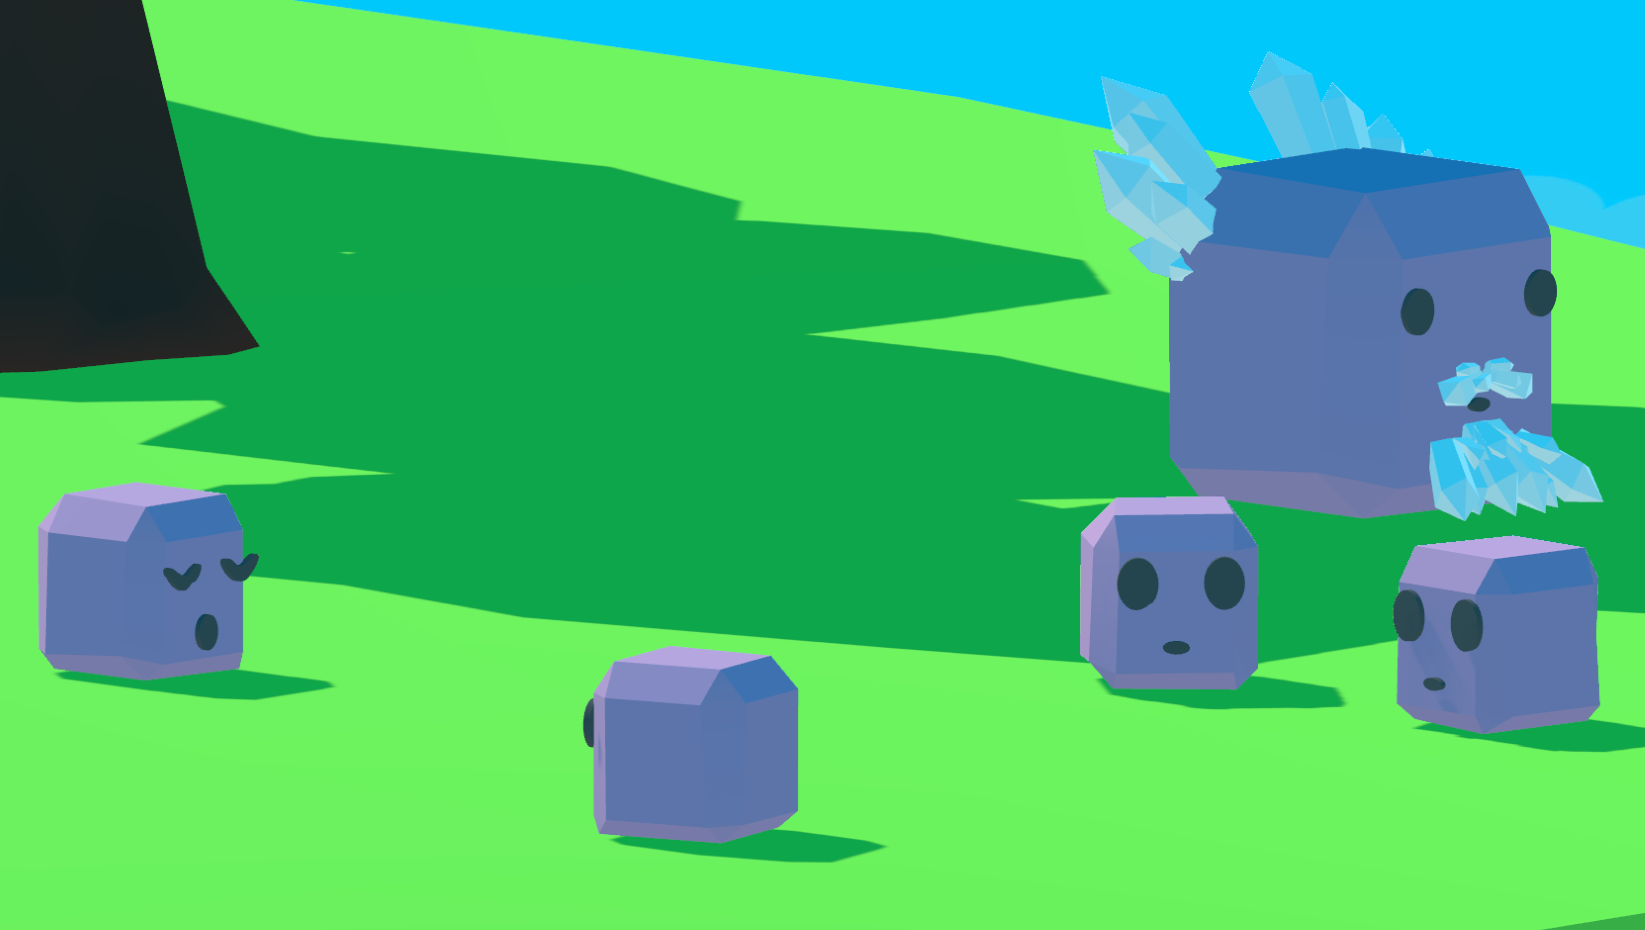
\includegraphics[height=6cm]{Environments/rockCreatures.png}
\caption{An image of the Rock creatures.}
\label{fig:rockCreatures}
\end{figure}

The Cherry creatures are organic by nature. They start their lives growing from the cherry trees. When they are mature, which is when they've grown to the size of a big coconut, they drop to the ground and start exploring their environment. They move by jumping around, which also makes them hard to catch, when they are not resting for a while. The size of the Cherry creatures makes them fit comfortably in the player's hands compared to the other creatures which are of larger nature.

\begin{figure}[h]
\centering
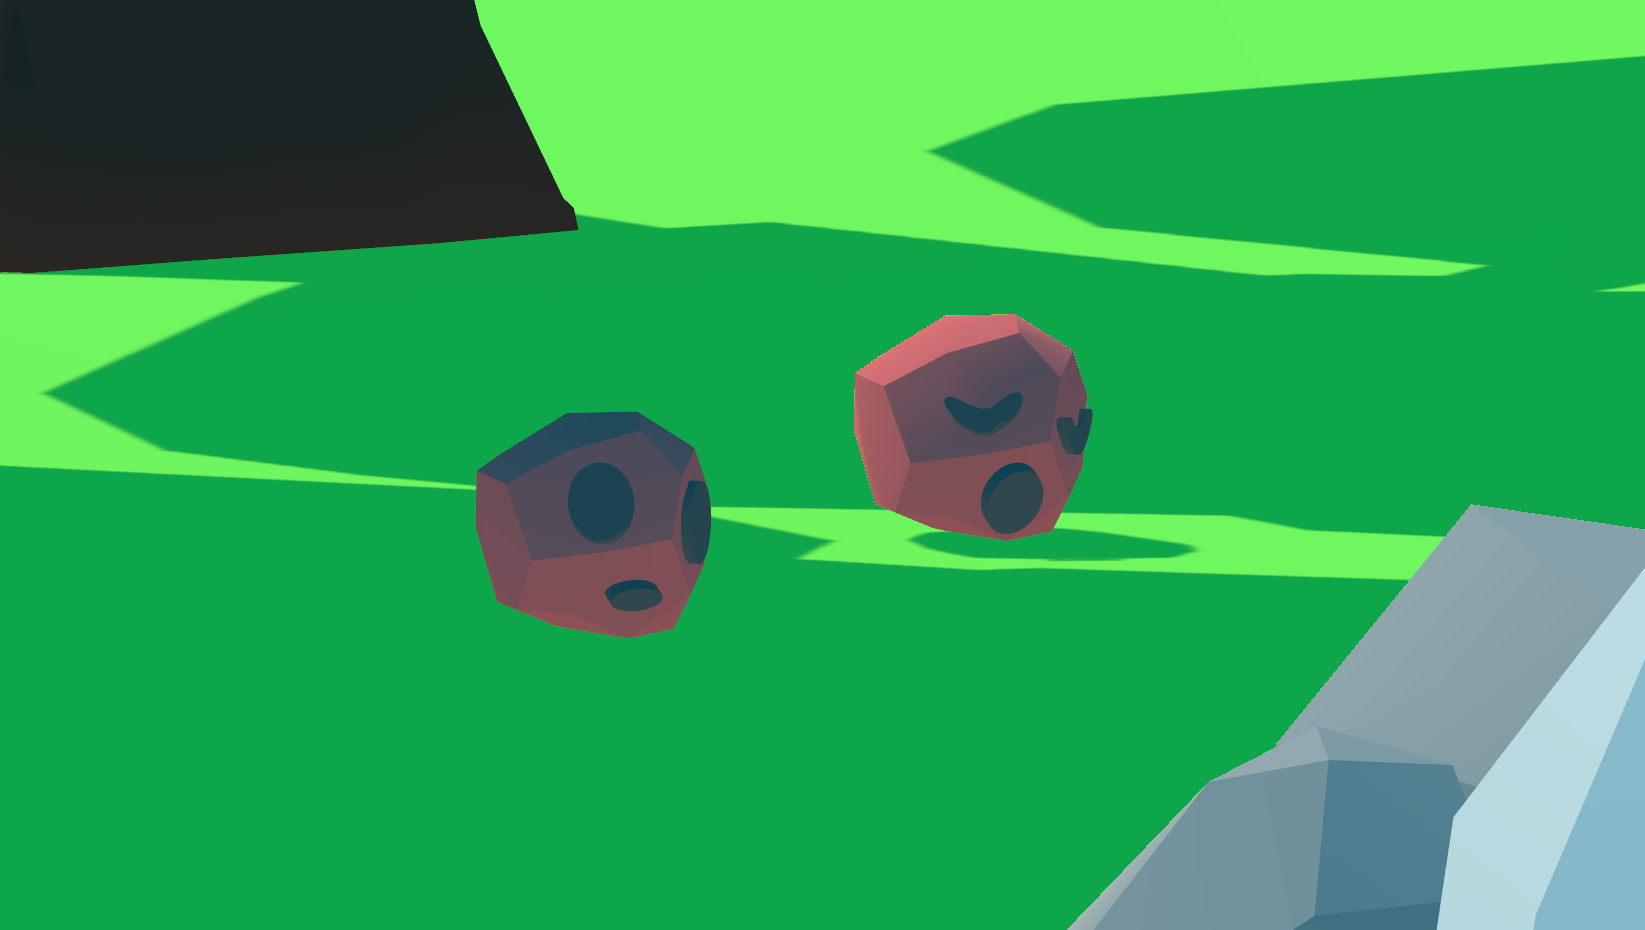
\includegraphics[height=6cm]{Environments/cherryCreatures.png}
\caption{An image of the Cherry creatures.}
\label{fig:cherryCreatures}
\end{figure}

The Mole creatures are capsule shaped creatures, who stick their heads out of their holes to have a look around. When touched or hit, they bounce up and down in a spring-like fashion, usually drawing players to hit them even more. When hit hard they even jump out of their holes completely. If grouped together, they could be compared to a game of whack-a-mole.  They only move in a straight line up and down, but can also spin around. They don't like being picked up though, so grabbing a Mole creature isn't an option. They would rather want to stay in their holes, although they do keep their heads poking out, while the player is still around on Touchy Island, to keep a watchful eye.

\begin{figure}[h]
\centering
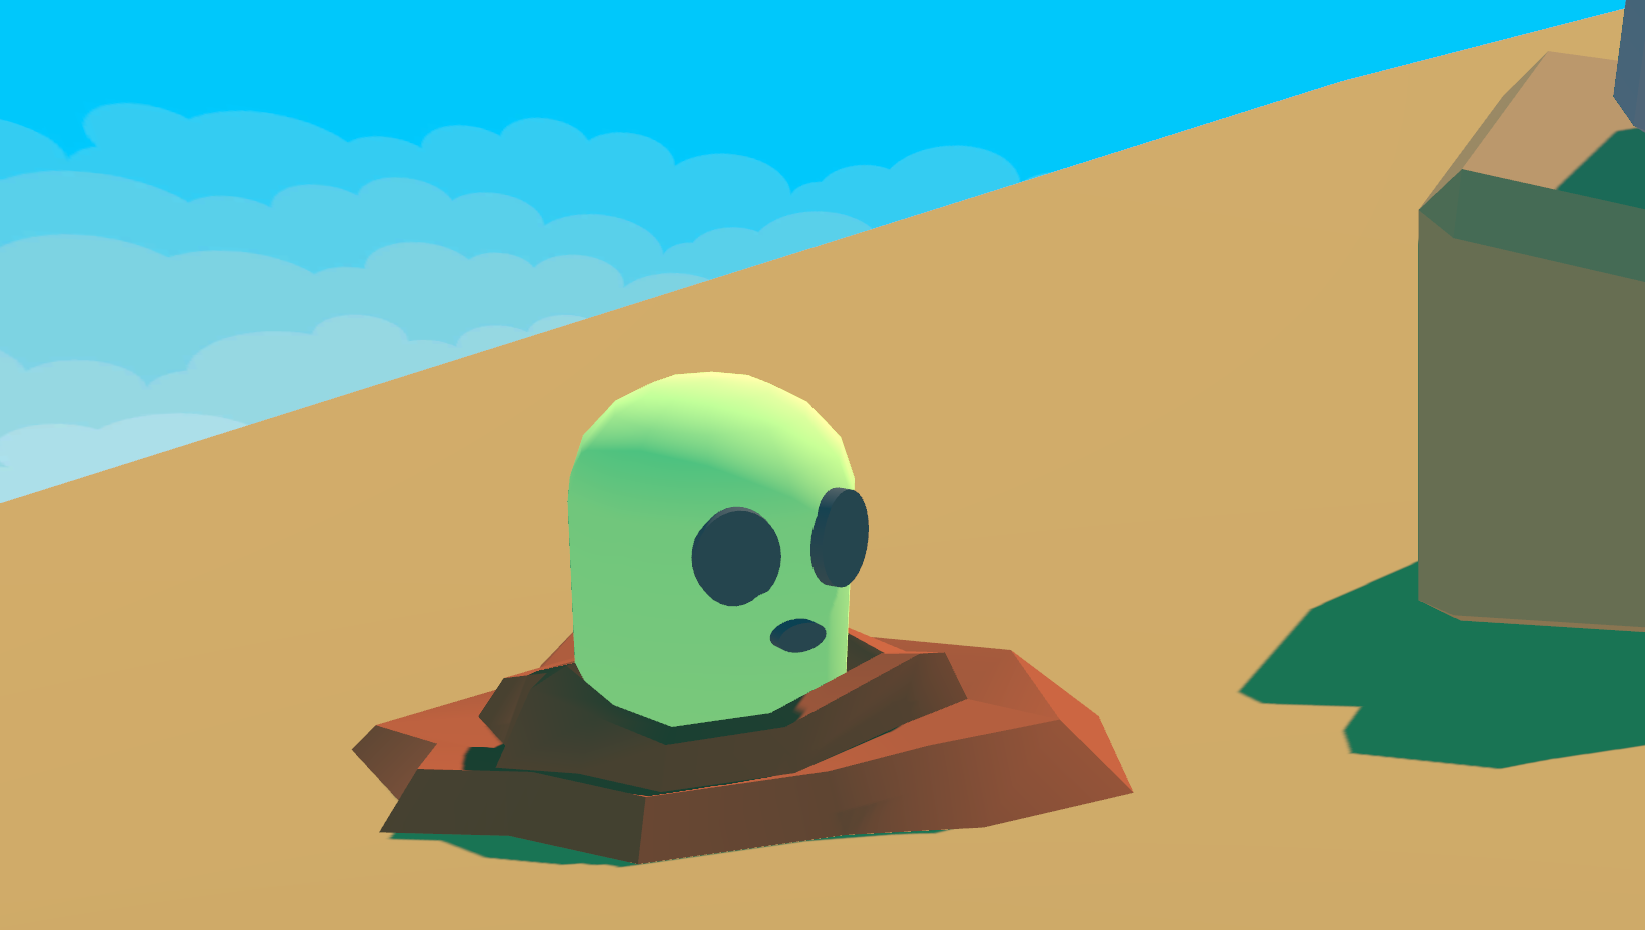
\includegraphics[height=6cm]{Environments/moleCreatures.png}
\caption{An image of the Mole creatures.}
\label{fig:moleCreatures}
\end{figure}

The Cloud creatures float around and are usually very happy. They can be pushed around if done lightly, but will always try to find a comfortable hovering height over the ground. The Cloud creatures are extremely delicate and can't handle hard hits or grabs. If the player chooses to grab or hit a cloud creature they are killed in a poof of smoke. So in order for the player to interact with the cloud creature they need to employ a light touch.

\begin{figure}[h]
\centering
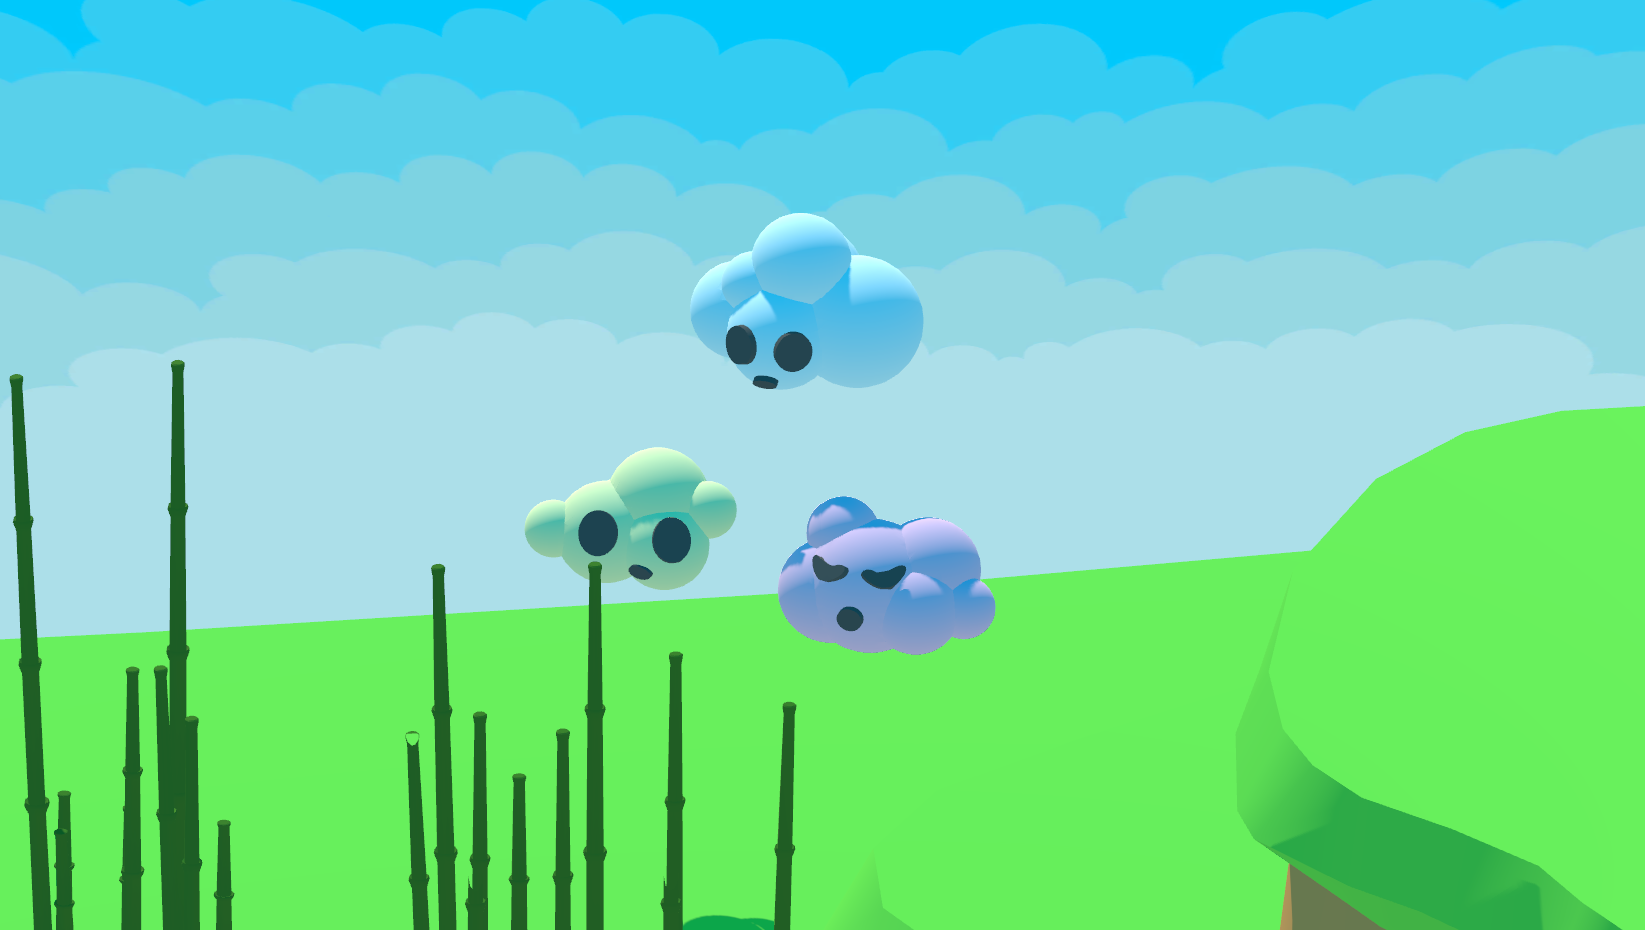
\includegraphics[height=6cm]{Environments/cloudCreatures.png}
\caption{An image of the Cloud creatures.}
\label{fig:cloudCreatures}
\end{figure}

The creatures all have moods which are affected by their surroundings. Creatures can be in one of four different moods: Neutral, Happy, Sad and Angry. Each of these moods are represented in a creature by a value, which most of the time is between 0 and 100. A creature's current mood is always decided by whichever of the Happy, Sad and Angry values are the highest, except if none of them have a value above 50 in which case their mood is Neutral. Some creature's moods are affected over time, slowly increasing or decreasing. These values can be defined for each individual creature, although we chose values that in general were close to each other with slight modifications for the different creature types. The main factor which can change a creature's mood is the player's actions. If a player is gentle and strokes or pets a creature they will become increasingly happy, up till a point where they might even start singing spreading their joy to other nearby creatures. On the other hand, if the player is throwing or hitting a creature it will become sadder and angrier and surrounding creatures will become sad. The easiest way to make creatures sad is to throw one of their friends over the edge of the island or to poof a cloud by hitting or grabbing it, resulting in their death. A creature's current mood is displayed by their facial expression. Creatures all have a face, which can look neutral, happy, sad or angry. Along with that, they also have temporary facial expressions which display the effect of an action. When petted for a while a creature's eyes will turn into hearts, for instance. This way the creatures give the player feedback on the effect of their actions.

As mentioned above there are also two interactive objects besides the creatures. They both exist to allow the player to experience different interactions. The interactive objects are bamboos and movable rocks. On the island there is a small bamboo forest. If the player so desires, they can break off the bamboo from its root and use it as a stick to throw, push or hit things with. The bamboos are connected to their roots using joints which have a certain break force. This allows the player to be able to grab the bamboo and then pull it off its root, but they can also be hit to break them. The movable rocks are essentially just rocks that are spread around the island but aren't stuck in the ground. We disabled the grabbing feature from the rocks and made them rather heavy so that players could experience the different feel of weight when pushing and lifting the rocks with the different hands. Finally, the island also has static objects like small crystals, immovable rocks, the cherry trees and some plateaus. When the player interacts with these they'll really see the position filtering in action for the Physics hand along with the real hand visualization and notice the fact that our implementation of the Job Simulator hand moves straight through such objects. 

\begin{figure}[h]
\centering
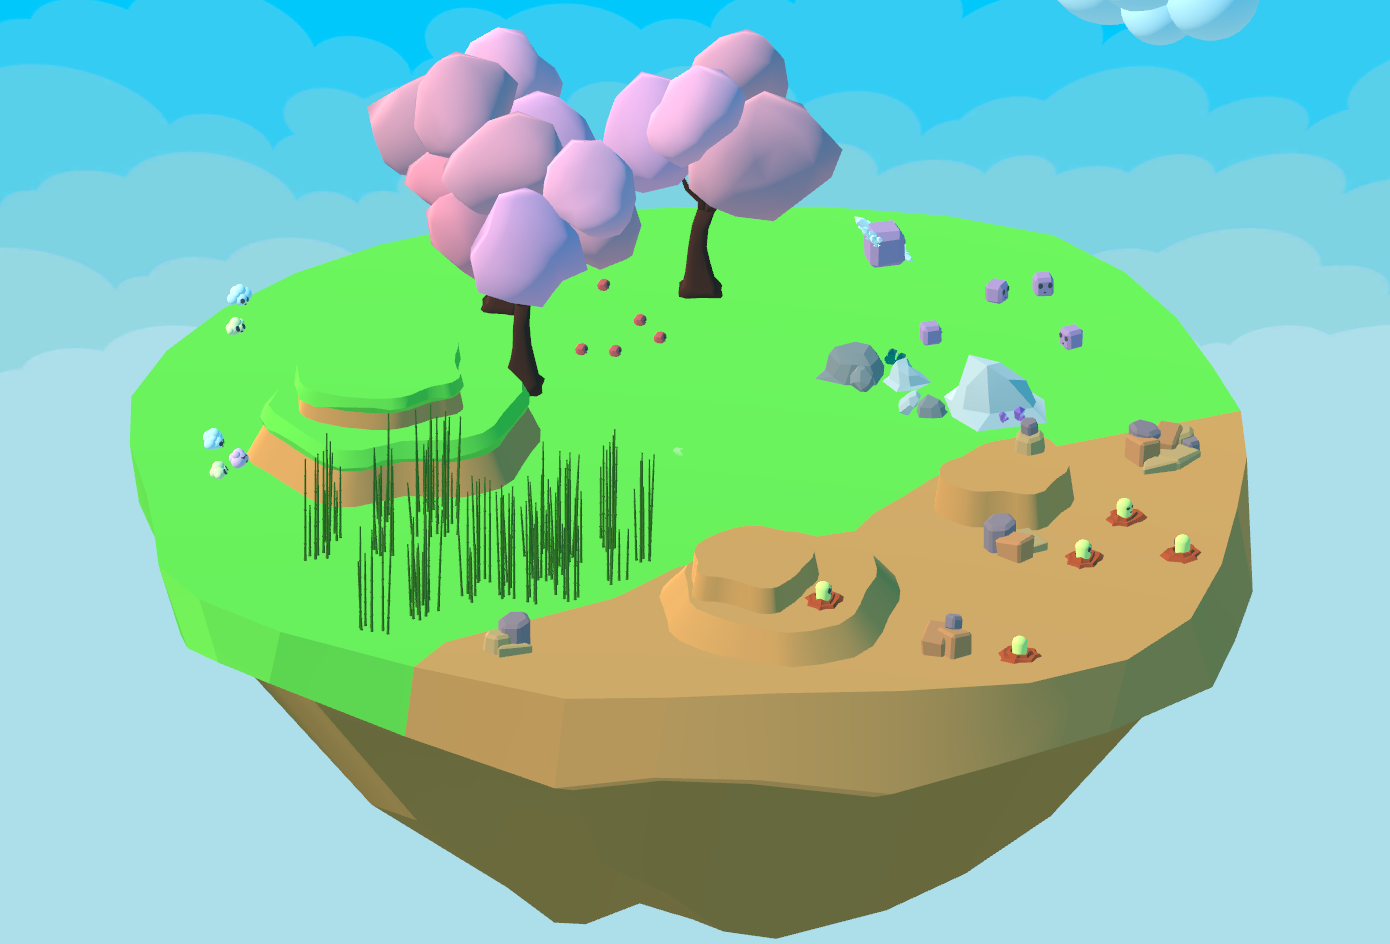
\includegraphics[height=10cm]{Environments/touchyIsland.png}
\caption{An image of Touchy Island.}
\label{fig:touchyIsland}
\end{figure}

All these different creatures and objects all have their distinct purpose in the world because of their unique features. These are not only implemented to have diversity, but also to draw in the player and make them want to interact with the environment. The reason for the creatures to have moods that are affected by the player's actions is to make the players want to interact and thereby use the hands. This also leads back into the decision to make a more game-like experience than another stale test environment. By first having testers go through the guided tour that is the Dev World evaluation and learn the features of the hand, releasing them into this playful sandbox would be a different experience which was more in-context of where the hands might be used in a real game. By having two evaluations, one in each of these different environments, we hoped that players would get an increased understanding of the hands and their use as well as more impressions of their functionality. 
